\section{Preventivo}
\label{Preventivo}

La sezione Preventivo ha lo scopo di stimare il costo complessivo della realizzazione del progetto. \\ 
La suddivisione oraria segue alcune regole comuni per ogni membro:
\begin{enumerate}

	\item I componenti dovranno svolgere tutti i ruoli almeno una volta;
	\item Ogni componente dovrà lavorare almeno 8 ore per ogni ruolo;
	\item Tutti i componenti avranno lo stesso numero di ore di lavoro ad ogni revisione.

\end{enumerate}
Per facilitare la lettura delle tabelle sono state scelte delle sigle da inserire in esse, rappresentanti i ruoli da ricoprire:
\begin{itemize}
	\item RE: \textit{Responsabile};
	\item AM: \textit{Amministratore};
	\item AN: \textit{Analista};
	\item PJ: \textit{Progettista};
	\item PR: \textit{Programmatore};
	\item VE: \textit{Verificatore}.
\end{itemize}

\newpage
\subsection{Avvio ed Analisi dei Requisiti}
\label{PAAR}
\subsubsection{Prospetto Orario}

Nel periodo di \textit{Avvio ed Analisi dei Requisiti} la suddivisione oraria, per ogni membro del gruppo, è la seguente:

\begin{longtable}{|C{.30\textwidth}|C{.06\textwidth}|C{.06\textwidth}|C{.06\textwidth} | C{.06\textwidth}| C{.06\textwidth} | C{.06\textwidth} | C{.10\textwidth} |}
\hline
\rowcolor{bluelogo}	\textbf{\textcolor{white}{Nome}} & \textbf{\textcolor{white}{RE}} & \textbf{\textcolor{white}{AM}} & \textbf{\textcolor{white}{AN}} & \textbf{\textcolor{white}{PJ}} & \textbf{\textcolor{white}{PR}} & \textbf{\textcolor{white}{VE}} & \textbf{\textcolor{white}{Totale}}\\
\hline 
Marco Chilese & - & - & 10 & - & - & 15 & 25 \\
\hline
\rowcolor{grigio}Marco Favaro & - & - & 14 & - & - & 11 & 25 \\
\hline
Diego Mazzalovo & - & - & 18 & - & - & 7 & 25 \\
\hline
\rowcolor{grigio}Carlotta Segna & 13 & - & - & - & - & 12 & 25 \\
\hline
Matteo Slanzi & - & 10 & 8 & - & - & 7 & 25 \\
\hline
\rowcolor{grigio}Bogdan Stanciu & 15 & - & 10 & - & - & - & 25\\
\hline
Luca Violato & - & 15 & 10 & - & - & - & 25 \\
\hline


\caption{Distribuzione oraria nel periodo di Avvio ed Analisi dei Requisiti}
\label{tab:dist oraria aar}
\end{longtable}
Il seguente grafico dà una visione della suddivisione dei ruoli per il primo periodo di \textit{Avvio ed Analisi dei Requisiti}:
\begin{figure}[H]
	\centering
  		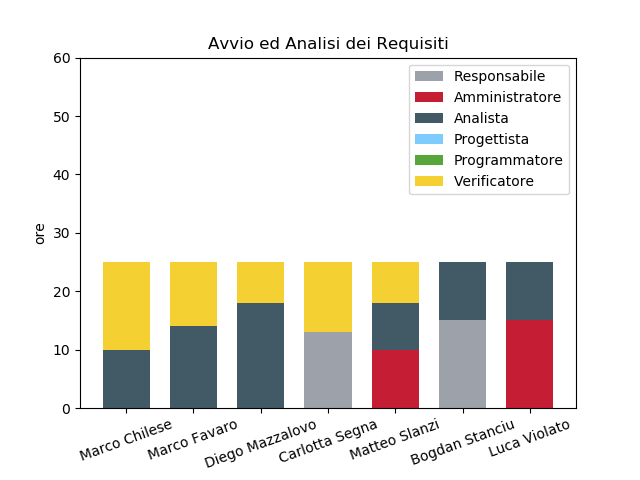
\includegraphics[width=0.8\linewidth]{./images/fig_aar.png}
  		\caption{Grafico suddivisione ore per persona nel periodo di Avvio ed Analisi dei Requisiti}
  		\label{fig:grafico suddivione ruoli aar}
\end{figure}



\subsubsection{Prospetto Economico}
Nel periodo di \textit{Avvio ed Analisi dei Requisiti} la suddivisione oraria, per quanto riguarda i ruoli, è la seguente: 

\begin{longtable}{| C{.30\textwidth}| C{.15\textwidth}| C{.20\textwidth}|}
\hline
\rowcolor{bluelogo}\textbf{\textcolor{white}{Ruolo}} & \textbf{\textcolor{white}{Ore}} & \textbf{\textcolor{white}{Costo in \euro}} \\
\hline
Responsabile & 28 & \EUR{840.00} \\
\hline
\rowcolor{grigio}Amministratore & 25 & \EUR{500.00} \\
\hline
Analista & 70 & \EUR{1750.00} \\
\hline
\rowcolor{grigio}Progettista & - & - \\
\hline
Programmatore & - & - \\
\hline
\rowcolor{grigio}Verificatore & 52 & \EUR{780.00}\\
\hline
\textbf{Totale} & 175 & \EUR{3870.00} \\
\hline

\caption{Distribuzione oraria dei ruoli nel periodo di Avvio ed Analisi dei Requisiti}
\label{tab: distribuzione oraria aar}
\end{longtable}

Il seguente grafico dà una rappresentazione visiva della suddivisione dei ruoli:
\begin{figure}[H]
	\centering
  		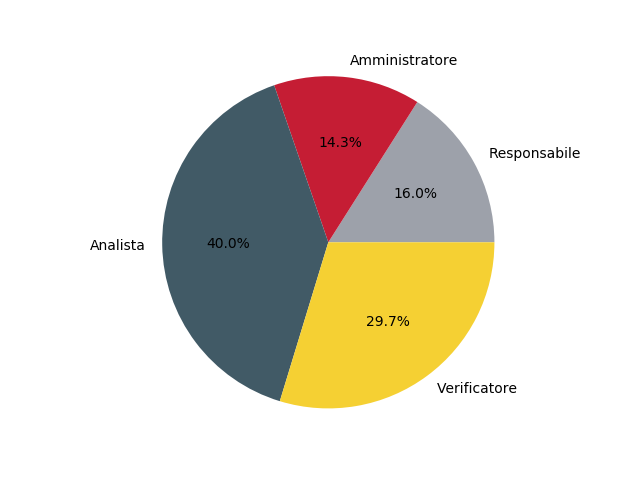
\includegraphics[width=1\linewidth]{./images/torta_aar.png}
  		\caption{Grafico suddivisione ruoli nel periodo di Avvio ed Analisi dei Requisiti}
  		\label{fig:grafico suddivione ruoli periodo di Avvio ed analisi dei requisiti}
\end{figure}

\newpage
\subsection{Risanamento Criticità}
\label{PRC1}
\subsubsection{Prospetto Orario}

Nel primo periodo di \textit{Risanamento delle Criticità} la suddivisione oraria, per quanto riguarda i ruoli, è la seguente:

\begin{longtable}{|C{.30\textwidth}|C{.06\textwidth}|C{.06\textwidth}|C{.06\textwidth} | C{.06\textwidth}| C{.06\textwidth} | C{.06\textwidth} | C{.10\textwidth} |}
\hline
\rowcolor{bluelogo}	\textbf{\textcolor{white}{Nome}} & \textbf{\textcolor{white}{RE}} & \textbf{\textcolor{white}{AM}} & \textbf{\textcolor{white}{AN}} & \textbf{\textcolor{white}{PJ}} & \textbf{\textcolor{white}{PR}} & \textbf{\textcolor{white}{VE}} & \textbf{\textcolor{white}{Totale}}\\
\hline 
Marco Chilese & - & - & - & - & - & 5 & 5 \\
\hline
\rowcolor{grigio}Marco Favaro & - & - & 5 & - & - & - & 5 \\
\hline
Diego Mazzalovo & - & - & 5 & - & - & - & 5 \\
\hline
\rowcolor{grigio}Carlotta Segna & - & - & - & - & - & 5 & 5 \\
\hline
Matteo Slanzi & - & - & 5 & - & - & - & 5 \\
\hline
\rowcolor{grigio}Bogdan Stanciu & 5 & - & - & - & - & - & 5 \\
\hline
Luca Violato & - & 5 & - & - & - & - & 5 \\
\hline

\caption{Distribuzione oraria nel periodo di Risanamento Criticità 1}
\label{Distribuzione oraria del periodo di rc1}
\end{longtable}



Il seguente grafico dà una visione della suddivisione dei ruoli per il primo periodo di \textit{Risanamento delle Criticità}:
\begin{figure}[H]
  \centering
  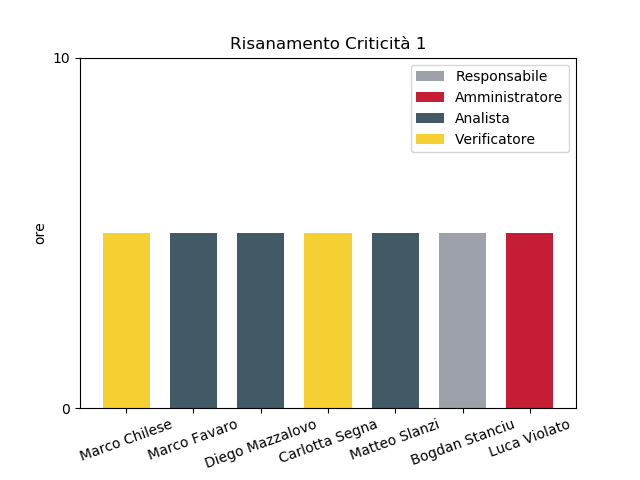
\includegraphics[width=0.8\linewidth]{./images/fig_rc1.png}
  \caption{Grafico suddivisione ore per persona nel periodo di Risanamento Criticità 1}
  \label{fig:grafico suddivione ruoli rc1}
\end{figure}

\subsubsection{Prospetto Economico}
Nel primo periodo di \textit{Risanamento delle Criticità} la suddivisione oraria, per quanto riguarda i ruoli, è la seguente: 


\begin{longtable}{| C{.30\textwidth}| C{.15\textwidth}| C{.20\textwidth}|}
\hline
\rowcolor{bluelogo}\textbf{\textcolor{white}{Ruolo}} & \textbf{\textcolor{white}{Ore}} & \textbf{\textcolor{white}{Costo in \euro}} \\
\hline 
Responsabile & 5 & \EUR{150.00} \\
\hline
\rowcolor{grigio}Amministratore & 5 & \EUR{100.00} \\
\hline
Analista & 15 & \EUR{375.00} \\
\hline
\rowcolor{grigio}Progettista & - & - \\
\hline
Programmatore & - & - \\
\hline
\rowcolor{grigio}Verificatore & 10 & \EUR{150.00}\\
\hline
\textbf{Totale} & 35 & \EUR{775.00} \\
\hline


\caption{Distribuzione oraria dei ruoli nel periodo di Risanamento Criticità 1}
\label{Distribuzione oraria ruoli del periodo di rc1}
\end{longtable}

Il seguente grafico dà una rappresentazione visiva della suddivisione dei ruoli:
\begin{figure}[H]
	\centering
  		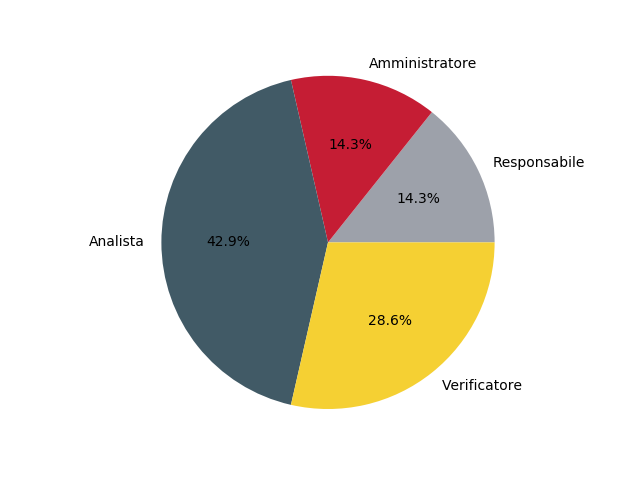
\includegraphics[width=1\linewidth]{./images/torta_rc1.png}
  		\caption{Grafico suddivisione ruoli nel periodo di Risanamento Criticità 1}
  		\label{fig:grafico suddivione ruoli periodo di rc1}
\end{figure}

\newpage
\subsection{Progettazione Architetturale}
\label{PPA}
\subsubsection{Prospetto Orario}

Nel periodo di \textit{Progettazione Architetturale} la suddivisione oraria, per ogni membro del gruppo, è la seguente:


\begin{longtable}{|C{.30\textwidth}|C{.06\textwidth}|C{.06\textwidth}|C{.06\textwidth} | C{.06\textwidth}| C{.06\textwidth} | C{.06\textwidth} | C{.10\textwidth} |}
\hline
\rowcolor{bluelogo}	\textbf{\textcolor{white}{Nome}} & \textbf{\textcolor{white}{RE}} & \textbf{\textcolor{white}{AM}} & \textbf{\textcolor{white}{AN}} & \textbf{\textcolor{white}{PJ}} & \textbf{\textcolor{white}{PR}} & \textbf{\textcolor{white}{VE}} & \textbf{\textcolor{white}{Totale}}\\
\hline 
Marco Chilese & - & 10 & - & 12 & - & - & 22 \\
\hline
\rowcolor{grigio}Marco Favaro & 5 & - & 17 & - & - & - & 22 \\
\hline
Diego Mazzalovo & 8 & - & - & 14 & - & - & 22 \\ 
\hline
\rowcolor{grigio}Carlotta Segna & - & - & - & 10 & 12 & - & 22 \\
\hline
Matteo Slanzi & - & - & - & - & 11 & 11 & 22 \\
\hline
\rowcolor{grigio}Bogdan Stanciu & - & 10 & - & - & 12 & - & 22 \\
\hline
Luca Violato & - & - & 10 & - & - & 12 & 22 \\
\hline 

\caption{Distribuzione oraria del periodo di Progettazione Architetturale}
\label{Distribuzione oraria del periodo di pa}
\end{longtable}

Il seguente grafico dà una visione della suddivisione dei ruoli per il periodo di \textit{Progettazione Architetturale}:

\begin{figure}[H]
	\centering
  		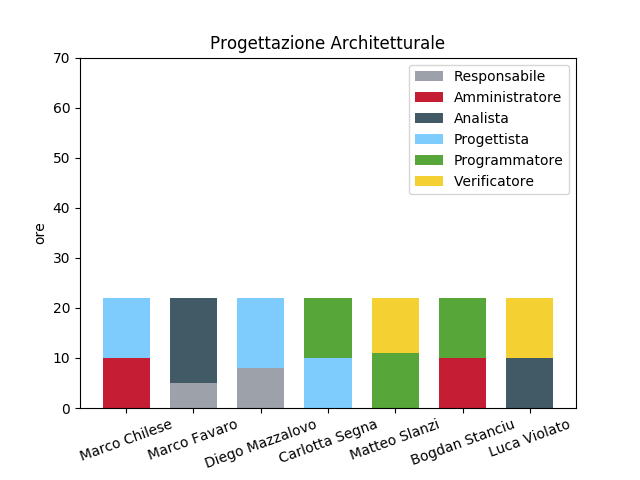
\includegraphics[width=0.8\linewidth]{./images/fig_pa.png}
  		\caption{Grafico suddivisione ore per persona nel periodo di Progettazione Architetturale}
  		\label{fig:grafico suddivione ruoli periodo di pa}
\end{figure}



\subsubsection{Prospetto Economico}
Nel periodo di \textit{Progettazione Architetturale} la suddivisione oraria, per quanto riguarda i ruoli, è la seguente: 


\begin{longtable}{| C{.30\textwidth}| C{.15\textwidth}| C{.20\textwidth}|}
\hline
\rowcolor{bluelogo}\textbf{\textcolor{white}{Ruolo}} & \textbf{\textcolor{white}{Ore}} & \textbf{\textcolor{white}{Costo in \euro}} \\
\hline 
Responsabile & 13 & \EUR{390.00} \\
\hline
\rowcolor{grigio}Amministratore & 20 & \EUR{400.00}\\
\hline
Analista & 27 & \EUR{675.00} \\
\hline
\rowcolor{grigio}Progettista & 36 & \EUR{792.00} \\
\hline
Programmatore & 35 & \EUR{525.00} \\
\hline
\rowcolor{grigio}Verificatore & 23 & \EUR{345.00} \\
\hline
\textbf{Totale} & 154 & \EUR{3127.00}\\ 
\hline

\caption{Distribuzione oraria dei ruoli nel periodo di Progettazione Architetturale}
\label{Distribuzione oraria per ruoli del periodo di pa}
\end{longtable}

Il seguente grafico dà una rappresentazione visiva della suddivisione dei ruoli:
\begin{figure}[H]
	\centering
  		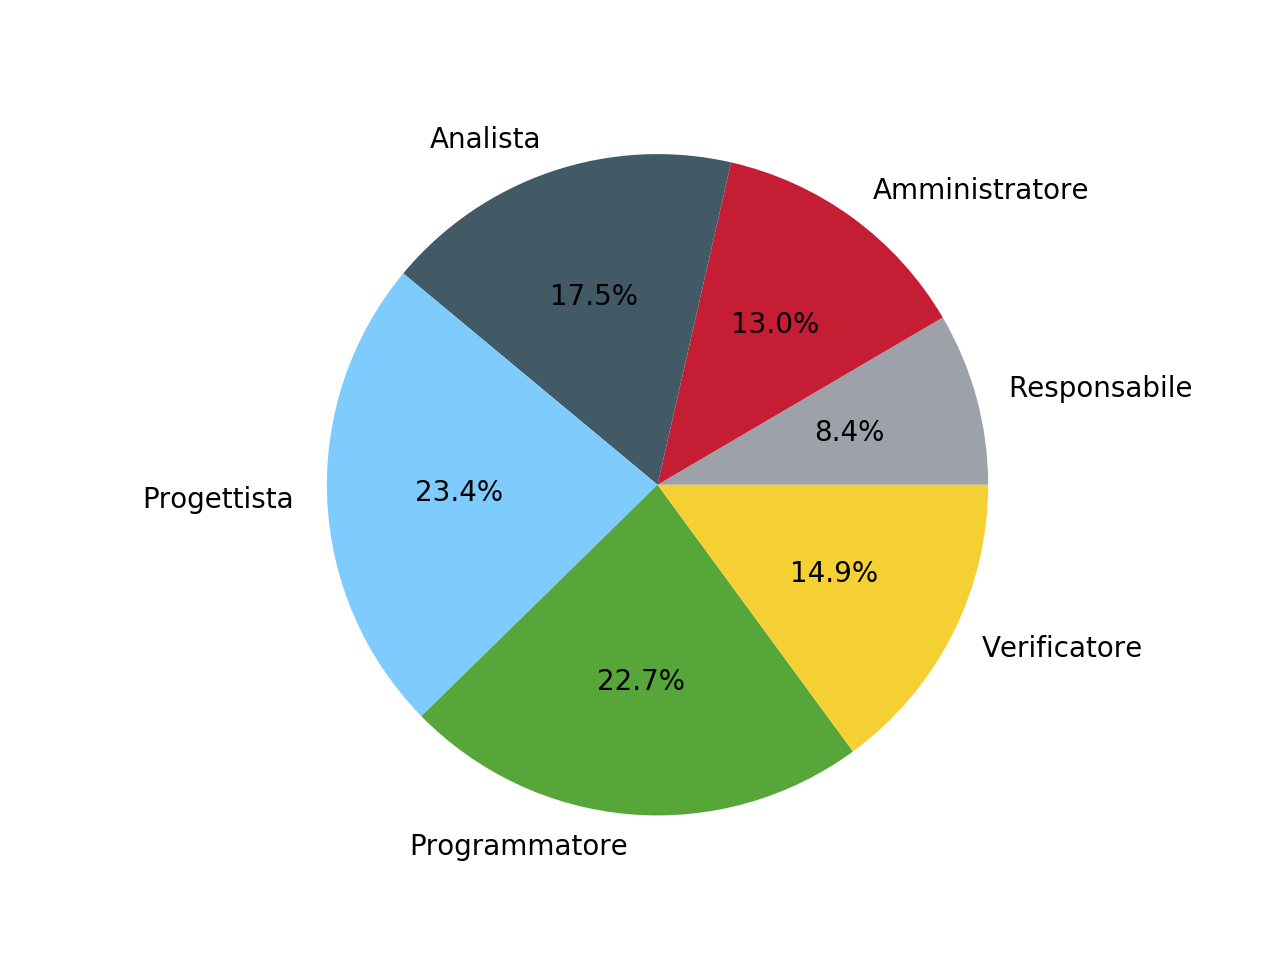
\includegraphics[width=1\linewidth]{./images/torta_pa.png}
  		\caption{Grafico suddivisione ruoli nel periodo di Progettazione Architetturale}
  		\label{fig:grafico suddivione ruoli pa}
\end{figure}

\newpage
\subsection{Risanamento Criticità}
\label{PRC2}

\subsubsection{Prospetto Orario}
Nel secondo periodo di \textit{Risanamento delle Criticità} la suddivisione oraria, per quanto riguarda i ruoli, è la seguente: 


\begin{longtable}{|C{.30\textwidth}|C{.06\textwidth}|C{.06\textwidth}|C{.06\textwidth} | C{.06\textwidth}| C{.06\textwidth} | C{.06\textwidth} | C{.10\textwidth} |}
\hline
\rowcolor{bluelogo}	\textbf{\textcolor{white}{Nome}} & \textbf{\textcolor{white}{RE}} & \textbf{\textcolor{white}{AM}} & \textbf{\textcolor{white}{AN}} & \textbf{\textcolor{white}{PJ}} & \textbf{\textcolor{white}{PR}} & \textbf{\textcolor{white}{VE}} & \textbf{\textcolor{white}{Totale}}\\
\hline 
Marco Chilese & - & 3 & - & - & - & - & 3 \\
\hline
\rowcolor{grigio}Marco Favaro & 3 & - & - & - & - & - & 3 \\
\hline
Diego Mazzalovo & - & - & - & 3 & - & - & 3 \\
\hline
\rowcolor{grigio}Carlotta Segna & - & - & - & - & 3 & - & 3 \\
\hline
Matteo Slanzi & - & - & - & - & - & 3 & 3 \\
\hline
\rowcolor{grigio}Bogdan Stanciu & - & - & 3 & - & - & - & 3 \\
\hline
Luca Violato & - & - & - & - & - & 3 & 3 \\   
\hline


\caption{Distribuzione oraria del periodo di Risanamento Criticità 2}
\label{Distribuzione oraria rc2}
\end{longtable}

Il seguente grafico dà una visione grafica della suddivisione dei ruoli per il secondo periodo di \textit{Risanamento delle Criticità}:\begin{figure}[H]
	\centering
  		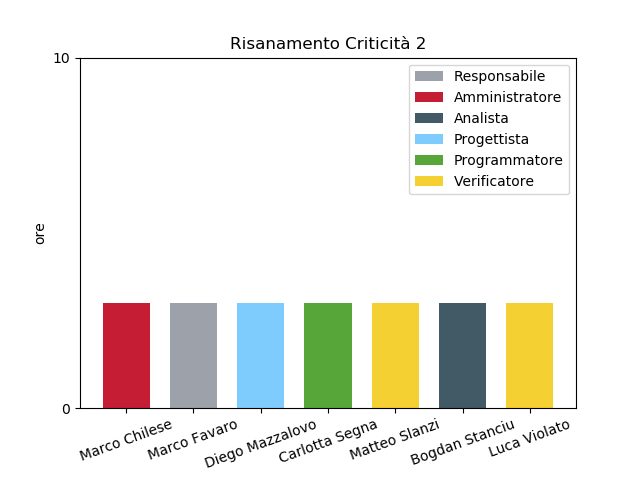
\includegraphics[width=0.8\linewidth]{./images/fig_rc2.png}
  		\caption{Grafico suddivisione ore per persona nel periodo di Risanamento Criticità 2}
  		\label{fig:grafico suddivione ruoli rc2}
\end{figure}



\subsubsection{Prospetto Economico}
Nel secondo periodo di \textit{Risanamento delle Criticità} la suddivisione oraria, per quanto riguarda i ruoli, è la seguente: 


\begin{longtable}{| C{.30\textwidth}| C{.15\textwidth}| C{.20\textwidth}|}
\hline
\rowcolor{bluelogo}\textbf{\textcolor{white}{Ruolo}} & \textbf{\textcolor{white}{Ore}} & \textbf{\textcolor{white}{Costo in \euro}} \\
\hline 
Responsabile & 3 & \EUR{90.00} \\
\hline
\rowcolor{grigio}Amministratore & 3 & \EUR{60.00} \\
\hline
Analista & 3 & \EUR{75.00} \\
\hline
\rowcolor{grigio}Progettista & 3 & \EUR{66.00}\\
\hline
Programmatore & 3 & \EUR{45.00} \\
\hline 
\rowcolor{grigio}Verificatore & 6 & \EUR{90.00} \\
\hline
\textbf{Totale} & 21 & \EUR{426.00} \\
\hline 

\caption{Distribuzione oraria dei ruoli nel periodo di Risanamento Criticità 2}
\label{Distribuzione oraria per ruoli rc2}
\end{longtable}

Il seguente grafico dà una rappresentazione visiva della suddivisione dei ruoli:
\begin{figure}[H]
	\centering
  		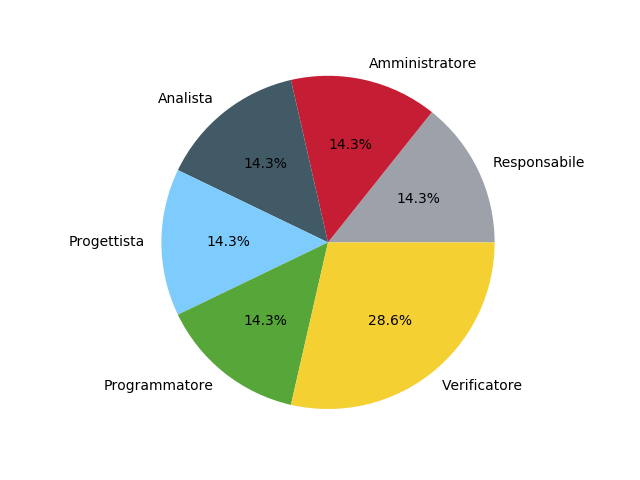
\includegraphics[width=1\linewidth]{./images/torta_rc2.png}
  		\caption{Grafico suddivisione ruoli nel periodo di Risanamento Criticità 2}
  		\label{fig:grafico suddivione ruoli rc2}
\end{figure}

\newpage
\subsection{Progettazione di Dettaglio e Codifica}
\label{PPDC}
\subsubsection{Prospetto Orario}

Nel periodo di \textit{Progettazione di Dettaglio e Codifica} la suddivisione oraria, per ogni membro del gruppo, è la seguente:

\begin{longtable}{|C{.30\textwidth}|C{.06\textwidth}|C{.06\textwidth}|C{.06\textwidth} | C{.06\textwidth}| C{.06\textwidth} | C{.06\textwidth} | C{.10\textwidth} |}
	\hline
	\rowcolor{bluelogo}	\textbf{\textcolor{white}{Nome}} & \textbf{\textcolor{white}{RE}} & \textbf{\textcolor{white}{AM}} & \textbf{\textcolor{white}{AN}} & \textbf{\textcolor{white}{PJ}} & \textbf{\textcolor{white}{PR}} & \textbf{\textcolor{white}{VE}} & \textbf{\textcolor{white}{Totale}}\\
	\hline 
	Marco Chilese & - & - & - & 20 & 16 & 14 & 50 \\
	\hline
	\rowcolor{grigio}Marco Favaro &  - & - & - & 14 & 19 & 17 & 50 \\
	\hline
	Diego Mazzalovo & - & 11 & - & 18 & 21 & - & 50 \\
	\hline
	\rowcolor{grigio}Carlotta Segna & - & 14 & 15 & - & 21 & - & 50 \\
	\hline
	Matteo Slanzi & 8 & - & - & 21 & 21 & - & 50 \\
	\hline
	\rowcolor{grigio}Bogdan Stanciu & - & - & 20 & 12 & - & 18 & 50 \\
	\hline
	Luca Violato & 5 & - & - & 22 & 23 & - & 50 \\   
	\hline


\caption{Distribuzione oraria nel periodo di Progettazione di Dettaglio e Codifica}
\label{Distribuzione oraria pdc}
\end{longtable}

Il seguente grafico dà una visione della suddivisione dei ruoli per il periodo di \textit{Progettazione di Dettaglio e Codifica}:

\begin{figure}[H]
	\centering
	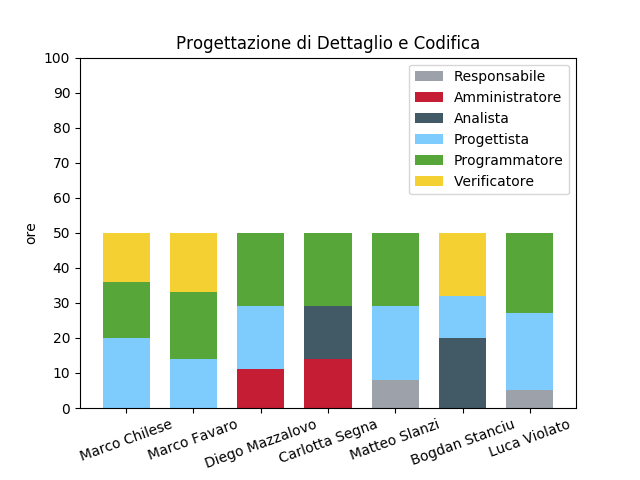
\includegraphics[width=0.8\linewidth]{./images/fig_pdc.png}
	\caption{Grafico suddivisione ore per persona nel periodo di Progettazione di Dettaglio e Codifica}
	\label{fig:grafico suddivione ruoli periodo pdc}
\end{figure}

\subsubsection{Prospetto Economico}

Nel periodo di \textit{Progettazione di Dettaglio e Codifica} la suddivisione oraria, per quanto riguarda i ruoli, è la seguente: 

\begin{longtable}{| C{.30\textwidth}| C{.15\textwidth}| C{.20\textwidth}|}
	\hline
	\rowcolor{bluelogo}\textbf{\textcolor{white}{Ruolo}} & \textbf{\textcolor{white}{Ore}} & \textbf{\textcolor{white}{Costo in \euro}} \\
	\hline 
	Responsabile & 13 & \EUR{390.00} \\
	\hline
	\rowcolor{grigio}Amministratore & 25 & \EUR{500.00}\\
	\hline
	Analista & 35 & \EUR{875.00} \\
	\hline
	\rowcolor{grigio}Progettista & 107 & \EUR{2354.00} \\
	\hline
	Programmatore & 121 & \EUR{1815.00} \\
	\hline
	\rowcolor{grigio}Verificatore & 49 & \EUR{735.00} \\
	\hline
	\textbf{Totale} & 350 & \EUR{6669.00}\\ 
	\hline
	
	\caption{Distribuzione oraria del periodo di Progettazione di Dettaglio e Codifica}
	\label{Distribuzione oraria dei ruoli pdc}
\end{longtable}

Il seguente grafico dà una rappresentazione visiva della suddivisione dei ruoli:
\begin{figure}[H]
	\centering
	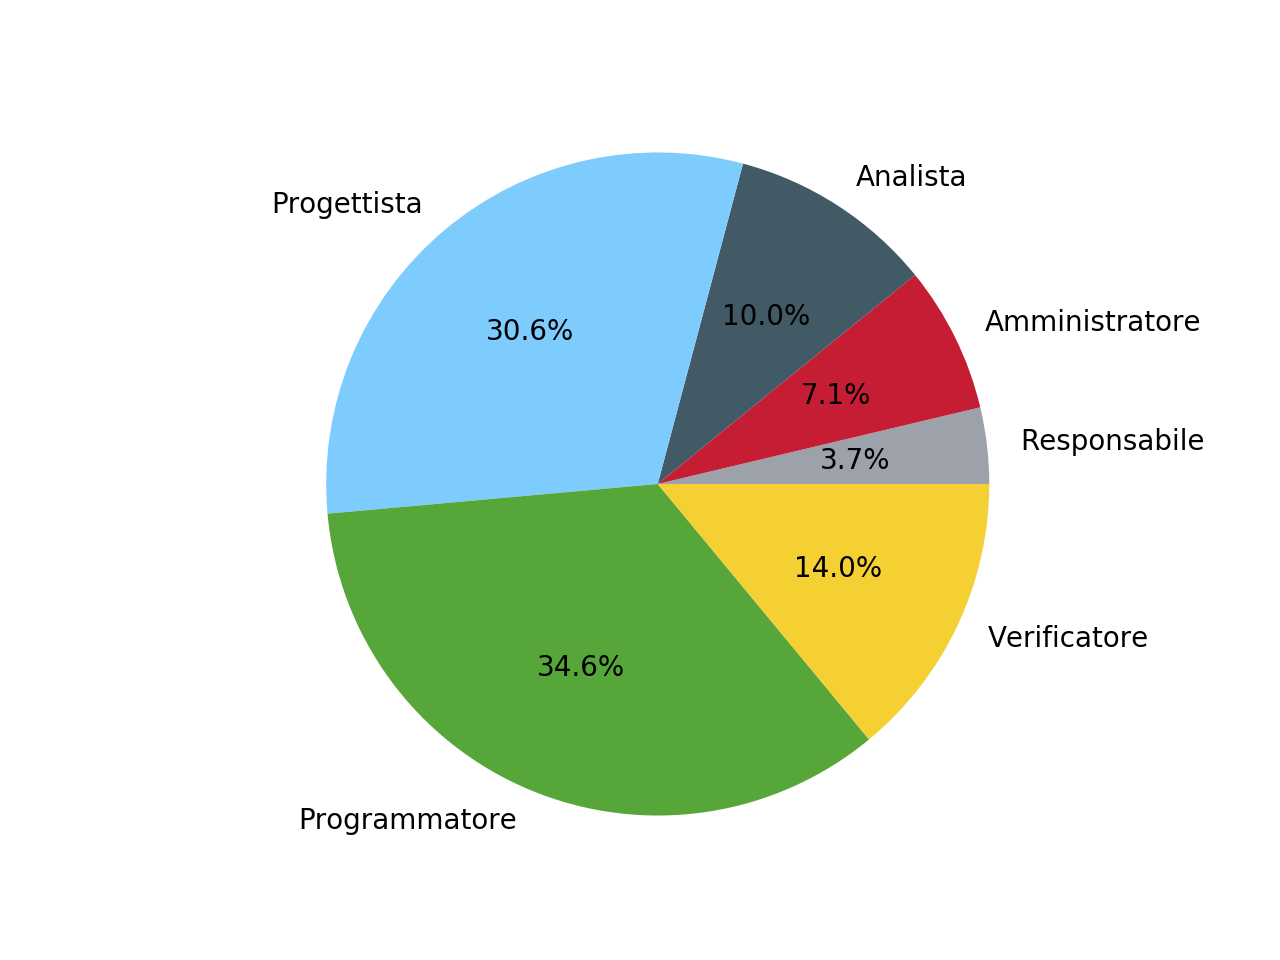
\includegraphics[width=1\linewidth]{./images/torta_pdc.png}
	\caption{Grafico suddivisione ore per persona nel periodo di Progettazione di Dettaglio e Codifica}
	\label{fig:grafico suddivione ruoli periodo pdc}
\end{figure}

\newpage
\subsection{Risanamento Criticità}
\label{PRC3}

\subsubsection{Prospetto Orario}
Nel terzo periodo di \textit{Risanamento delle Criticità} la suddivisione oraria, per ogni membro del gruppo, è la seguente:

\begin{longtable}{|C{.30\textwidth}|C{.06\textwidth}|C{.06\textwidth}|C{.06\textwidth} | C{.06\textwidth}| C{.06\textwidth} | C{.06\textwidth} | C{.10\textwidth} |}
\hline
\rowcolor{bluelogo}	\textbf{\textcolor{white}{Nome}} & \textbf{\textcolor{white}{RE}} & \textbf{\textcolor{white}{AM}} & \textbf{\textcolor{white}{AN}} & \textbf{\textcolor{white}{PJ}} & \textbf{\textcolor{white}{PR}} & \textbf{\textcolor{white}{VE}} & \textbf{\textcolor{white}{Totale}}\\
\hline 
	Marco Chilese & - & - & 3 & - & - & - & 3 \\
	\hline
	\rowcolor{grigio}Marco Favaro & - & - & - & - & - & 3 & 3 \\
	\hline
	Diego Mazzalovo & - & - & - & - & 3 & - & 3 \\
	\hline
	\rowcolor{grigio}Carlotta Segna & - & 3 & - & - & - & - & 3 \\
	\hline
	Matteo Slanzi & - & - & - & - & 3 & - & 3 \\
	\hline
	\rowcolor{grigio}Bogdan Stanciu & - & - & - & 3 & - & - & 3 \\
	\hline
	Luca Violato & 3 & - & - & - & - & - & 3 \\   
	\hline
	
	
	\caption{Distribuzione oraria del periodo di Risanamento Criticità 3}
	\label{Distribuzione oraria rc3}
\end{longtable}

Il seguente grafico dà una visione della suddivisione dei ruoli per il terzo periodo di  \textit{Risanamento delle Criticità}:\begin{figure}[H]
	\centering
	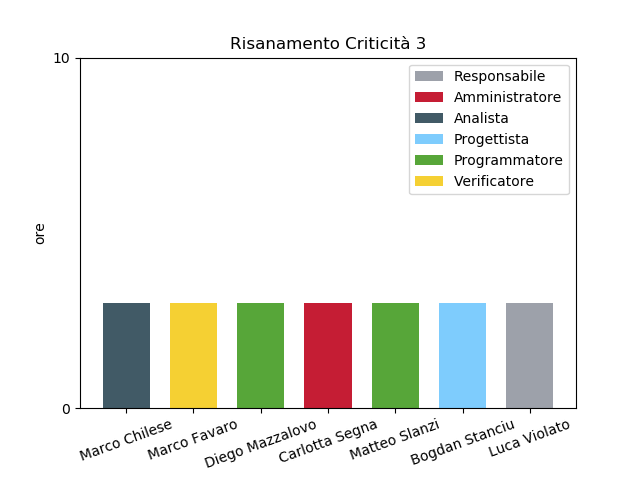
\includegraphics[width=0.8\linewidth]{./images/fig_rc3.png}
	\caption{Grafico suddivisione ore per persona nel periodo di Risanamento Criticità 3}
	\label{fig:grafico ore suddivione ruoli rc3}
\end{figure}

\subsubsection{Prospetto Economico}
Nel terzo periodo di \textit{Risanamento delle Criticità} la suddivisione oraria, per quanto riguarda i ruoli, è la seguente: 

\begin{longtable}{| C{.30\textwidth}| C{.15\textwidth}| C{.20\textwidth}|}
	\hline
	\rowcolor{bluelogo}\textbf{\textcolor{white}{Ruolo}} & \textbf{\textcolor{white}{Ore}} & \textbf{\textcolor{white}{Costo 	in \euro}} \\
	\hline 
	Responsabile & 3 & \EUR{90.00} \\
	\hline
	\rowcolor{grigio}Amministratore & 3 & \EUR{60.00} \\
	\hline
	Analista & 3 & \EUR{75.00} \\
	\hline
	\rowcolor{grigio}Progettista & 3 & \EUR{66.00}\\
	\hline
	Programmatore & 6 & \EUR{90.00} \\
	\hline 
	\rowcolor{grigio}Verificatore & 3 & \EUR{45.00} \\
	\hline
	\textbf{Totale} & 21 & \EUR{426.00} \\
	\hline 


\caption{Distribuzione oraria dei ruoli nel periodo di Risanamento Criticità 3}
\label{Distribuzione oraria per ruoli rc3}
\end{longtable}

Il seguente grafico dà una visione della suddivisione dei ruoli per il periodo di  \textit{Risanamento delle Criticità}:\begin{figure}[H]
	\centering
	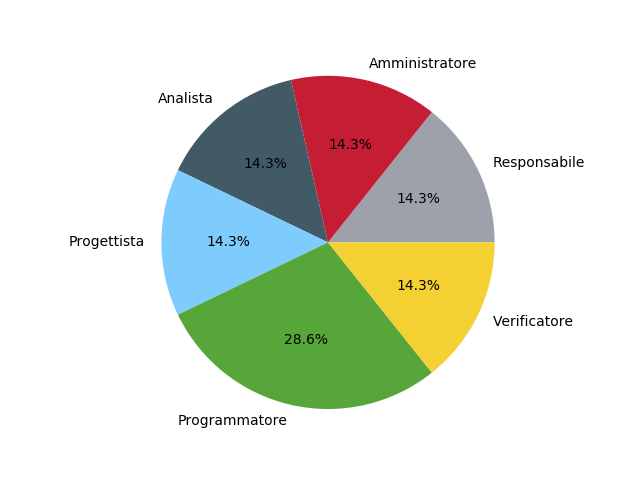
\includegraphics[width=1\linewidth]{./images/torta_rc3.png}
	\caption{Grafico suddivisione ruoli nel periodo di Risanamento Criticità 3}
	\label{fig:grafico suddivione ruoli rc3}
\end{figure}

\newpage
\subsection{Validazione e Collaudo}
\label{PVC}
\subsubsection{Prospetto Orario}
Nel periodo di \textit{Validazione e Collaudo} la suddivisione oraria, per ogni membro del gruppo, è la seguente:

\begin{longtable}{|C{.30\textwidth}|C{.06\textwidth}|C{.06\textwidth}|C{.06\textwidth} | C{.06\textwidth}| C{.06\textwidth} | C{.06\textwidth} | C{.10\textwidth} |}
	\hline
\rowcolor{bluelogo}	\textbf{\textcolor{white}{Nome}} & \textbf{\textcolor{white}{RE}} & \textbf{\textcolor{white}{AM}} & \textbf{\textcolor{white}{AN}} & \textbf{\textcolor{white}{PJ}} & \textbf{\textcolor{white}{PR}} & \textbf{\textcolor{white}{VE}} & \textbf{\textcolor{white}{Totale}}\\
	\hline 
	Marco Chilese & 8 & - & - & - & - & 14 & 22 \\
	\hline
	\rowcolor{grigio}Marco Favaro &  - & 10 & - & - & - & 12 & 22 \\
	\hline
	Diego Mazzalovo & - & - & - & - & 10 & 12 & 22 \\
	\hline
	\rowcolor{grigio}Carlotta Segna & - & - & - & - & 10 & 12 & 22 \\
	\hline
	Matteo Slanzi & - & - & - & 10 & - & 12 & 22 \\
	\hline
	\rowcolor{grigio}Bogdan Stanciu & - & - & - & 10 & - & 12 & 22 \\
	\hline
	Luca Violato & - & - & - & - & 10 & 12 & 22 \\   
	\hline
	
	
	\caption{Distribuzione oraria nel periodo di Validazione e Collaudo}
	\label{Distribuzione oraria vc}
\end{longtable}

Il seguente grafico dà una visione della suddivisione dei ruoli per il periodo di \textit{Validazione e Collaudo}:

\begin{figure}[H]
	\centering
	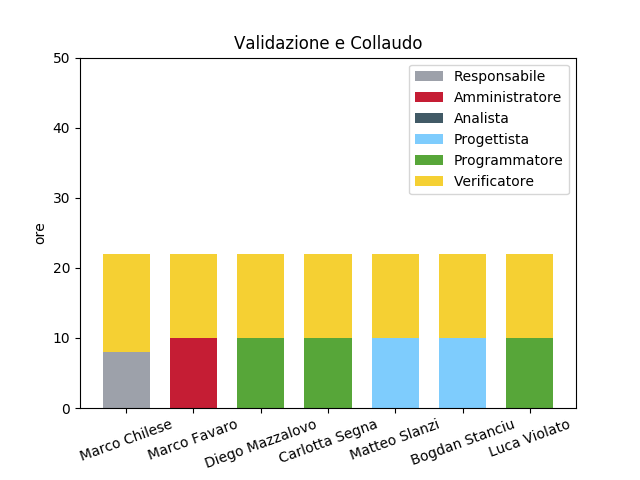
\includegraphics[width=0.8\linewidth]{./images/fig_vc.png}
	\caption{Grafico suddivisione ore per persona nel periodo di Validazione e Collaudo}
	\label{fig:grafico suddivione ruoli periodo vc}
\end{figure}


\subsubsection{Prospetto Economico}
Nel periodo di \textit{Validazione e Collaudo} la suddivisione oraria, per quanto riguarda i ruoli, è la seguente: 


\begin{longtable}{| C{.30\textwidth}| C{.15\textwidth}| C{.20\textwidth}|}
	\hline
	\rowcolor{bluelogo}\textbf{\textcolor{white}{Ruolo}} & \textbf{\textcolor{white}{Ore}} & \textbf{\textcolor{white}{Costo in \euro}} \\
	\hline 
	Responsabile & 8 & \EUR{240.00} \\
	\hline
	\rowcolor{grigio}Amministratore & 10 & \EUR{200.00}\\
	\hline
	Analista & 0 & \EUR{0.00} \\
	\hline
	\rowcolor{grigio}Progettista & 20 & \EUR{440.00} \\
	\hline
	Programmatore & 30 & \EUR{450.00} \\
	\hline
	\rowcolor{grigio}Verificatore & 86 & \EUR{1290.00} \\
	\hline
	\textbf{Totale} & 154 & \EUR{2620.00}\\ 
	\hline
	
	\caption{Distribuzione oraria dei ruoli nel periodo di Validazione e Collaudo}
	\label{Distribuzione oraria del periodo di Validazione e collaudo}
\end{longtable}

Il seguente grafico dà una rappresentazione visiva della suddivisione dei ruoli:
\begin{figure}[H]
	\centering
	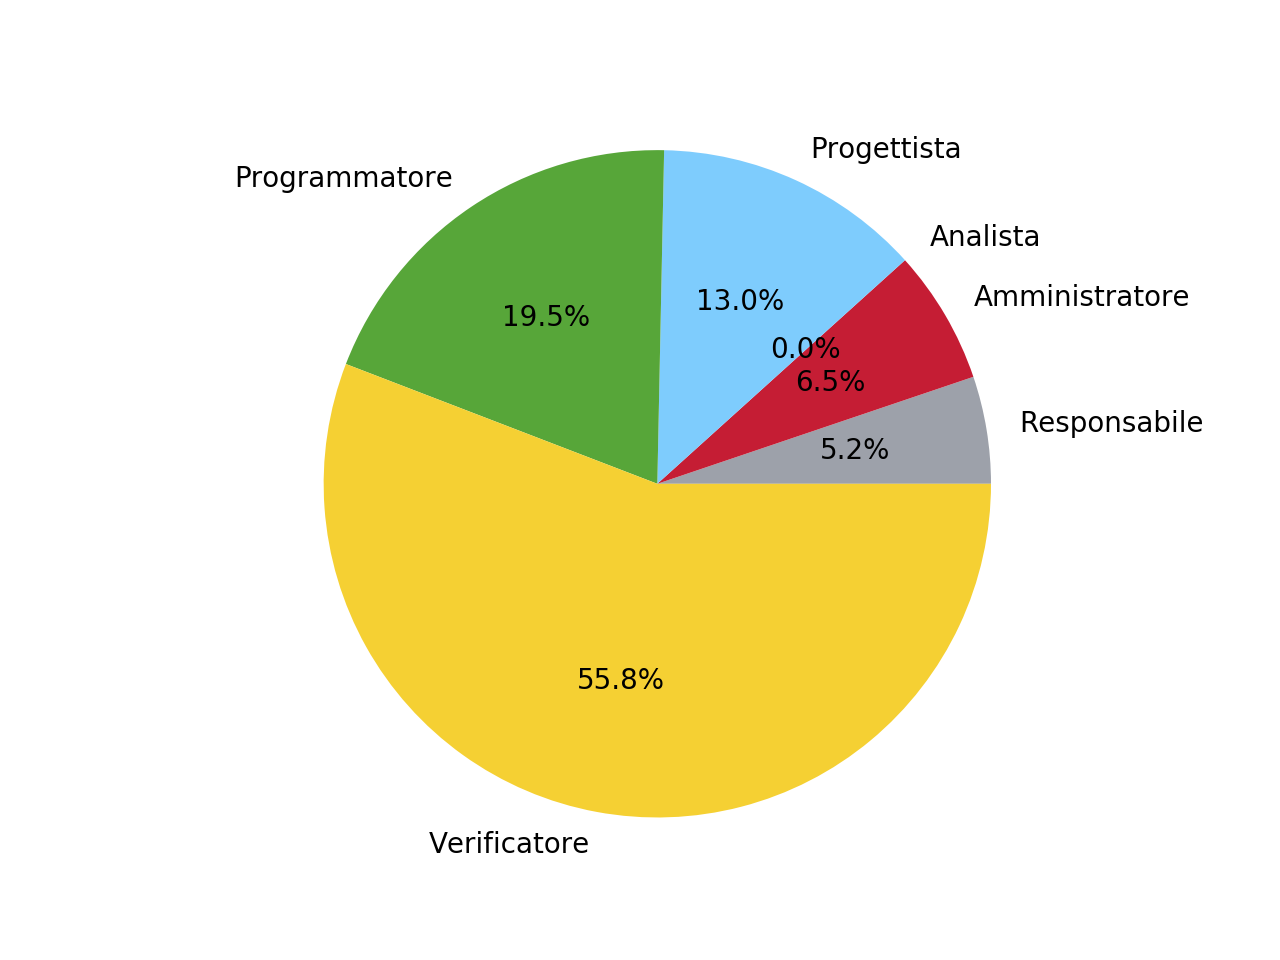
\includegraphics[width=1\linewidth]{./images/torta_vc.png}
	\caption{Grafico suddivisione ruoli nel periodo di Validazione e Collaudo}
	\label{fig:grafico suddivione ruoli periodo di Validazione e collaudo}
\end{figure}

\newpage
\subsection{Totale Ore Rendicontate}
\label{PTRR}
\subsubsection{Prospetto Orario}

Le ore di seguito riportate sono da considerarsi a carico del committente, le quali non includono le ore della prima fase:

\begin{longtable}{|C{.30\textwidth}|C{.06\textwidth}|C{.06\textwidth}|C{.06\textwidth} | C{.06\textwidth}| C{.06\textwidth} | C{.06\textwidth} | C{.10\textwidth} |}
\hline
\rowcolor{bluelogo}	\textbf{\textcolor{white}{Nome}} & \textbf{\textcolor{white}{RE}} & \textbf{\textcolor{white}{AM}} & \textbf{\textcolor{white}{AN}} & \textbf{\textcolor{white}{PJ}} & \textbf{\textcolor{white}{PR}} & \textbf{\textcolor{white}{VE}} & \textbf{\textcolor{white}{Totale}}\\
\hline 
Marco Chilese & 8 & 13 & 3 & 32 & 16 & 33 & 105\\
\hline
\rowcolor{grigio}Marco Favaro & 8 & 10 & 22 & 14 & 19 & 32 & 105\\
\hline
Diego Mazzalovo & 8 & 11 & 5 & 35 & 34 & 12 & 105\\
\hline
\rowcolor{grigio}Carlotta Segna & - & 17 & 15 & 10 & 46 & 17 & 105\\
\hline
Matteo Slanzi & 8 & - & 5 & 31 & 35 & 26 & 105\\
\hline
\rowcolor{grigio}Bodgan Stanciu & 5 & 10 & 23 & 25 & 12 & 30 & 105\\
\hline
Luca Violato & 8 & 5 & 10 & 22 & 33 & 27 & 105 \\
\hline

\caption{Distribuzione oraria delle ore Rendicontate}
\label{Distribuzione oraria delle ore rendicontate}
\end{longtable}

Il seguente grafico dà una visione della suddivisione dei ruoli complessiva:

\begin{figure}[H]
	\centering
  		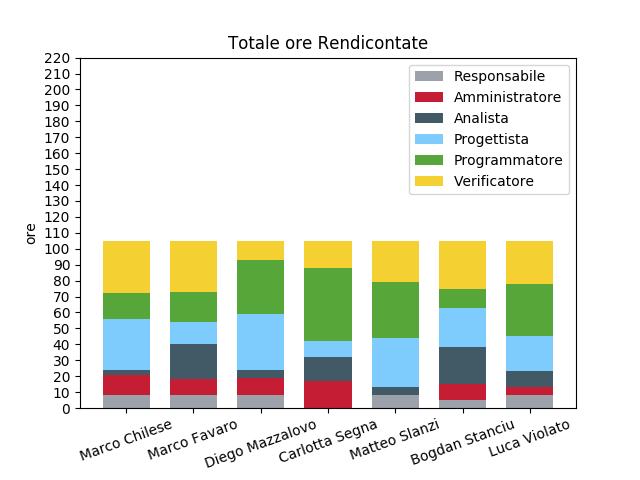
\includegraphics[width=0.8\linewidth]{./images/fig_tor.png}
  		\caption{Grafico suddivisione Ruoli Rendicontati}
  		\label{fig:grafico suddivione ruoli}
\end{figure}

\newpage

\subsubsection{Prospetto Economico}
Nel complesso la suddivisione oraria, per quanto riguarda i ruoli, è la seguente:

\begin{longtable}{| C{.30\textwidth}| C{.15\textwidth}| C{.20\textwidth}|}
\hline
\rowcolor{bluelogo}\textbf{\textcolor{white}{Ruolo}} & \textbf{\textcolor{white}{Ore}} & \textbf{\textcolor{white}{Costo in \euro}} \\
\hline \hline
\endhead
Responsabile & 45 & \EUR{1350.00} \\
\hline
\rowcolor{grigio}Amministratore & 66 & \EUR{1320.00} \\
\hline
Analista & 83 & \EUR{2075.00} \\
\hline
\rowcolor{grigio}Progettista & 169 & \EUR{3718.00}\\
\hline 
Programmatore & 195 & \EUR{2925.00} \\
\hline
\rowcolor{grigio}Verificatore & 177 & \EUR{2655.00} \\
\hline 
\textbf{Totale} & 735 & \EUR{14043.00}\\
\hline

\caption{Distribuzione oraria dei ruoli delle ore Rendicontate}
\label{Distribuzione oraria a carico del committente}
\end{longtable}

\begin{figure}[H]
	\centering
  		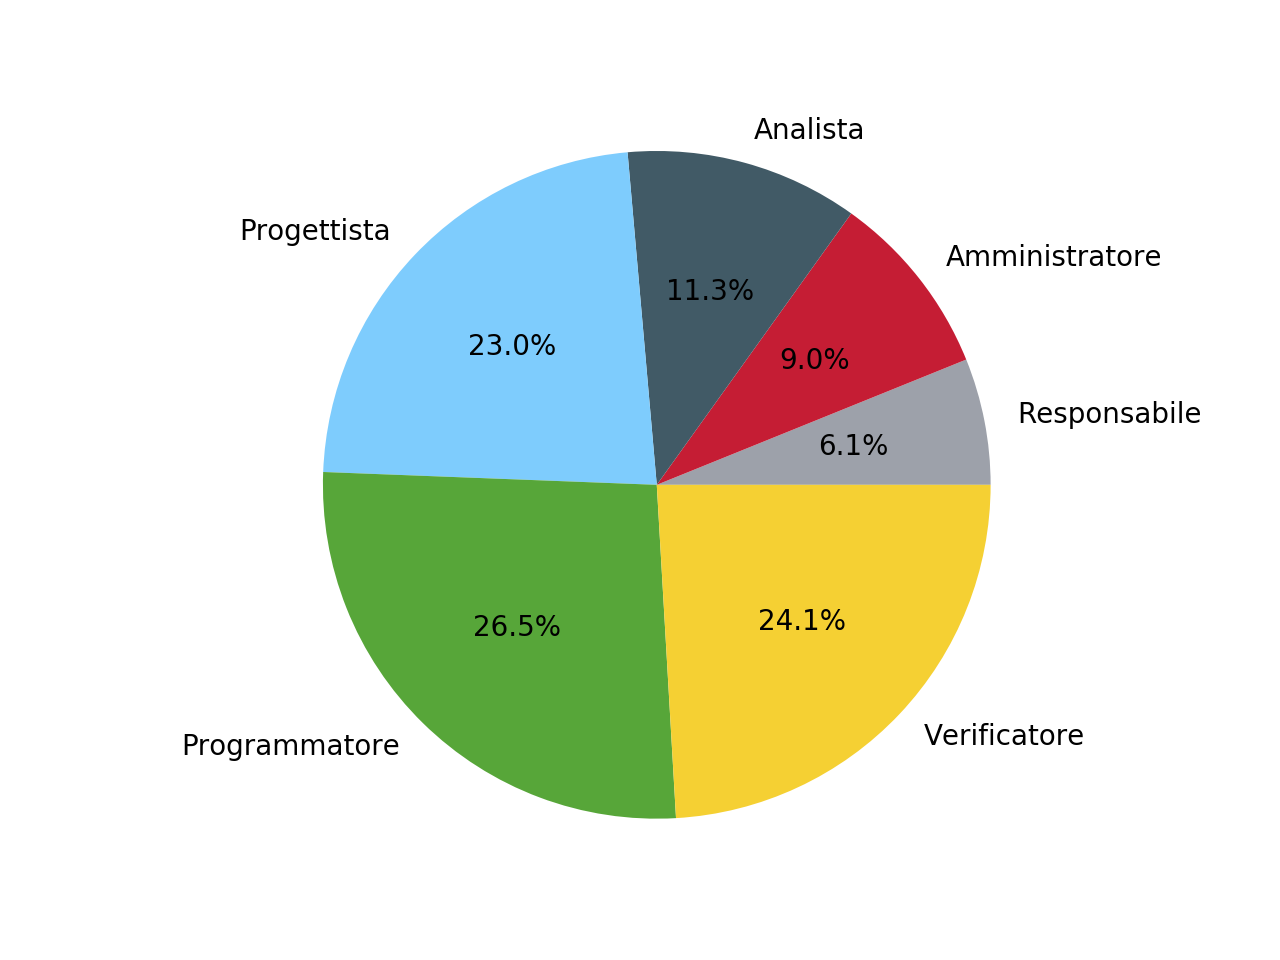
\includegraphics[width=1\linewidth]{./images/torta_to.png}
  		\caption{Grafico suddivisione Ruoli Rendicontati}
  		\label{fig:grafico suddivione ruoli}
\end{figure}


\newpage
\subsection{Totale Ore con Investimento}
\label{PTI}
\subsubsection{Prospetto Orario}

Le ore di seguito riportate sono comprensive delle ore di investimento da parte nostra, le quali includono le ore della prima fase:

\begin{longtable}{|C{.30\textwidth}|C{.06\textwidth}|C{.06\textwidth}|C{.06\textwidth} | C{.06\textwidth}| C{.06\textwidth} | C{.06\textwidth} | C{.10\textwidth} |}
\hline
\rowcolor{bluelogo}	\textbf{\textcolor{white}{Nome}} & \textbf{\textcolor{white}{RE}} & \textbf{\textcolor{white}{AM}} & \textbf{\textcolor{white}{AN}} & \textbf{\textcolor{white}{PJ}} & \textbf{\textcolor{white}{PR}} & \textbf{\textcolor{white}{VE}} & \textbf{\textcolor{white}{Totale}}\\
\hline 
Marco Chilese & 8 & 13 & 13 & 32 & 16 & 48 & 130\\
\hline
\rowcolor{grigio}Marco Favaro & 8 & 10 & 36 & 14 & 19 & 43 & 130\\
\hline
Diego Mazzalovo & 8 & 11 & 23 & 35 & 34 & 19 & 130\\
\hline
\rowcolor{grigio}Carlotta Segna & 13 & 17 & 15 & 10 & 46 & 29 & 130\\
\hline
Matteo Slanzi & 8 & 10 & 13 & 31 & 35 & 33 & 130\\
\hline
\rowcolor{grigio}Bodgan Stanciu & 20 & 10 & 33 & 25 & 12 & 30 & 130\\
\hline
Luca Violato & 8 & 20 & 20 & 22 & 33 & 27 & 130 \\
\hline


\caption{Distribuzione oraria con Investimento}
\label{Distribuzione oraria delle ore con investimento}
\end{longtable}

\begin{figure}[H]
	\centering
  		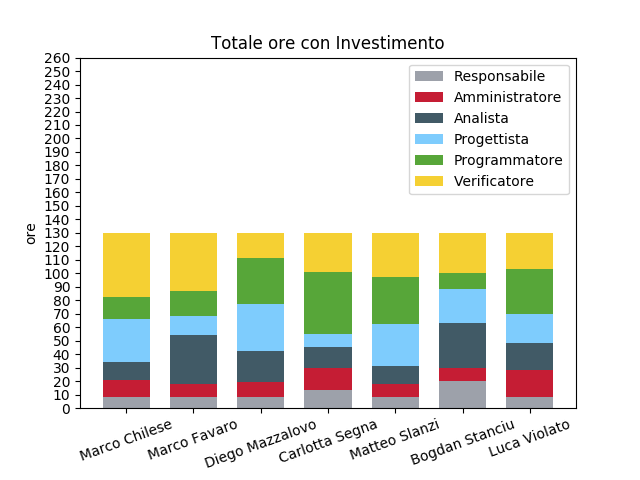
\includegraphics[width=0.8\linewidth]{./images/fig_toi.png}
  		\caption{Grafico suddivisione ruoli con Investimento}
  		\label{fig:grafico suddivione ruoli con investimento}
\end{figure}

\newpage

\subsubsection{Prospetto Economico}
Nel complesso la suddivisione oraria, per quanto riguarda i ruoli, è la seguente: 


\begin{longtable}{| C{.30\textwidth}| C{.15\textwidth}| C{.20\textwidth}|}
\hline
\rowcolor{bluelogo}\textbf{\textcolor{white}{Ruolo}} & \textbf{\textcolor{white}{Ore}} & \textbf{\textcolor{white}{Costo in \euro}} \\
\hline \hline
\endhead
Responsabile & 73 & \EUR{2190.00}\\
\hline
\rowcolor{grigio}Amministratore & 91 & \EUR{1820.00} \\
\hline
Analista & 153 & \EUR{3825.00} \\
\hline 
\rowcolor{grigio}Progettista & 169 & \EUR{3718.00}\\
\hline
Programmatore & 195 & \EUR{2925.00} \\
\hline
\rowcolor{grigio}Verificatore & 229 & \EUR{3435.00} \\
\hline
\textbf{Totale} & 910 & \EUR{17913.00} \\
\hline
\caption{Distribuzione oraria dei ruoli con Investimento}
\label{Distribuzione oraria ruoli con investimento}
\end{longtable}

\begin{figure}[H]
	\centering
  		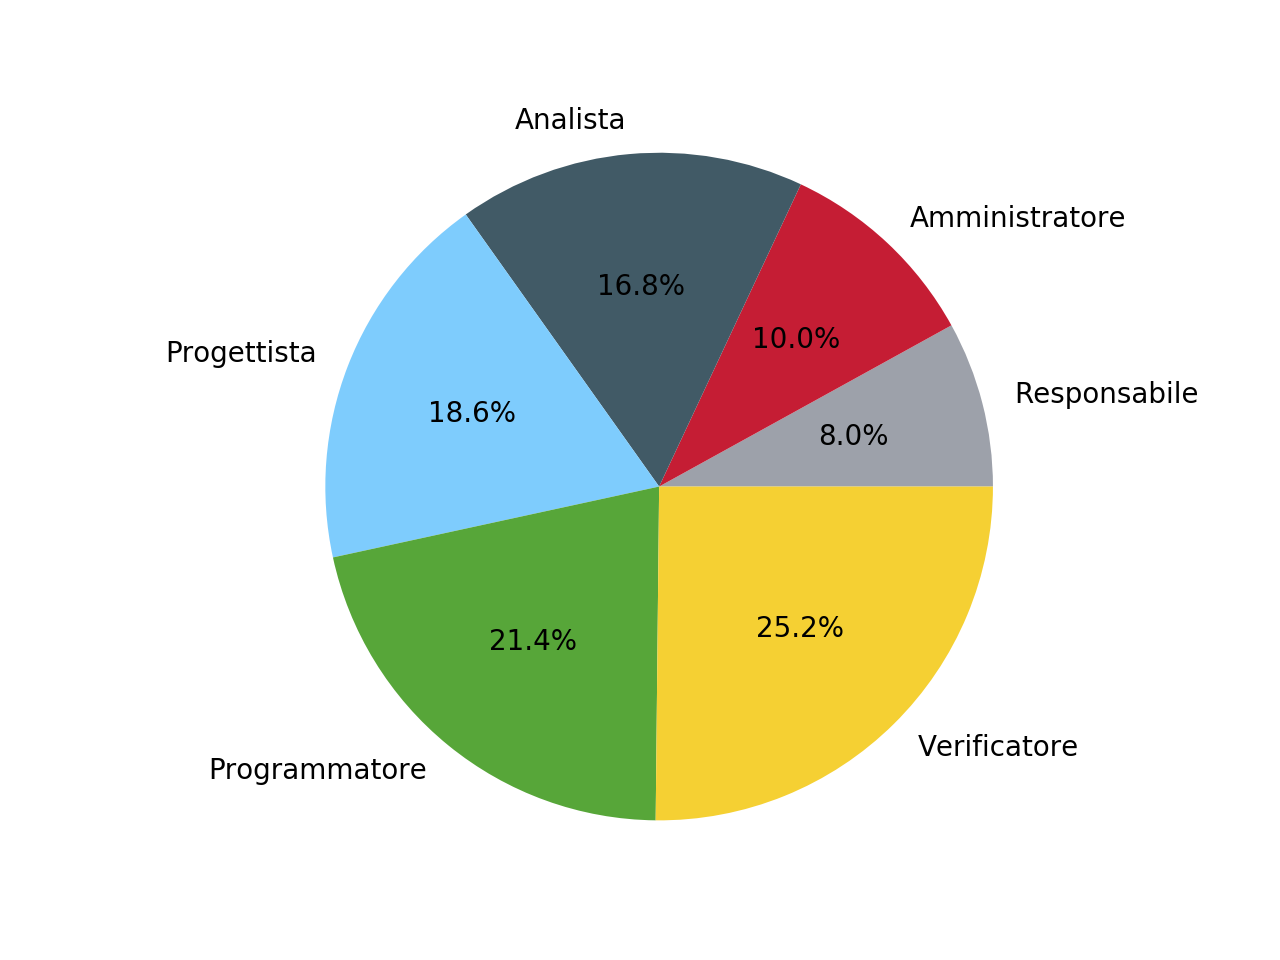
\includegraphics[width=1\linewidth]{./images/torta_toci.png}
  		\caption{Grafico suddivisione ruoli con Investimento}
  		\label{fig:grafico suddivione ruoli con investimento}
\end{figure}



